\subsection{Dataset}


For training a system to recognize facial expression effectively, the dataset should focus on several main expressions including anger, disgust, fear, happiness, sadness and surprise. Moreover, a proper dataset should be composed of faces with kinds of face shapes, colors, facial and scalp hairs from many participants with different genders, ethnic backgrounds and ages. 

\\
The dataset this paper adopted is from the Cohn-Kanade Facial Expression Dataset. The dataset refers to seven emotions including anger, contempt, disgust, fear, happiness, sadness and surprise. There are 5105 images from 123 subjects, who ranged in age from 18 to 30 years. Sixty-five percent are female, eight-five percent are Euro-American and fifteen percent are African-American and Asian. They were observed in an observation room equipped with a chair on which to sit and a camera was located directly in front of the subject. Therefore all images have the uniform background and lighting. The images were digitized into 640*480 or 490 pixel arrays with 8-bit precision for grayscale values and are available in png and jpg. 

\\
In the Cohn-Kanade Facial Expression Dataset, subjects performed a series of several facial displays from neutral expressions to peak expressions and images were taken frame by frame. In order to train a powerful system, we chose neutral faces and obvious expressions. That means there is no indistinguishable expression in our dataset. Figure 1 shows some example of the dataset.



\begin{figure}[h!]
\centering
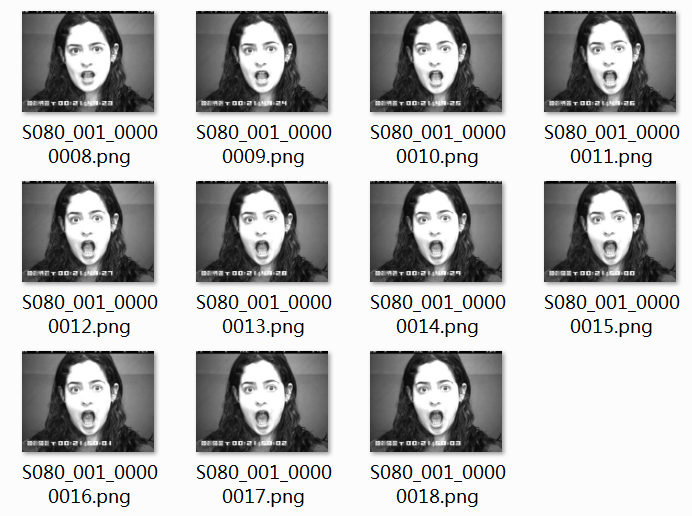
\includegraphics[scale=0.8]{example.png}
\caption{Example of dataset}
\label{Example of dataset}
\end{figure}